\chapter{The database}
\label{chapter:the-database}

\section{Database Model}
The logic behind the database is to keep track of reservations, customers, hotels, rooms and facilities.
The database is designed to handle reservations of rooms at hotels, and to keep track of customer information and what facilities the hotels offer.

This results in the database consisting of the following tables:
\begin{itemize}
  \item Hotels
  \item Customers
  \item Rooms
  \item Reservations
  \item Facilities
  \item HotelFacilities
\end{itemize}

\subsection{Relations and Multiplicity}

\begin{itemize}
  \item A Hotel can have many Rooms (1 to Many)
  \item A Customer can have many Reservations (1 to Many)
  \item A Room can be part of one Reservation at a time (1 to Many)
  \item Facilities are shared among Hotels through HotelFacilities (Many to Many)
\end{itemize}

\subsection{3NF State}
All tables are in 3NF because:
\begin{enumerate}
  \item They are in 1NF as all attributes are \emph{atomic} - no groups are repeated or contain more than one value.
      This can be seen, for example, by HotelFacilities being a relationship table between Hotel and Facility.
  \item They are in 2NF as there is no \emph{partial dependency} - Non-key columns depend solely on the PK.
      This can be seen, for example, by Hotel having a relationship to Facility instead of containing Facility as an attribute.
  \item There are no \emph{transitive dependencies} - Non-key columns depend only on the PK.
      This can be seen, for example, by Room having a relationship to Hotel instead of containing Hotel as an attribute.
\end{enumerate}

\section*{Diagrams}
The diagrams should be simple enough to be self-explanatory. The DMD is created first and based on the many-to-many relationship between hotels and facilities, it gives rise to an index table (HotelFacilities).
In the DMD, HotelFacilities is not considered as an independent entity but rather as a way to manage the relationship between Hotel and Facilities.

\begin{figure}
  \centering
  \begin{subfigure}[b]{0.45\textwidth}
    \centering
    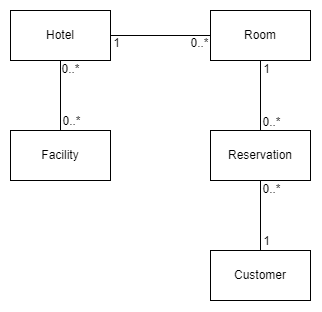
\includegraphics[width=\textwidth]{figures/SWD_Domain_HotelManagement.png}
    \caption{Domain Model Diagram}\label{DomainModelDiagram}
  \end{subfigure}
  \hfill
  \begin{subfigure}[b]{0.45\textwidth}
    \centering
    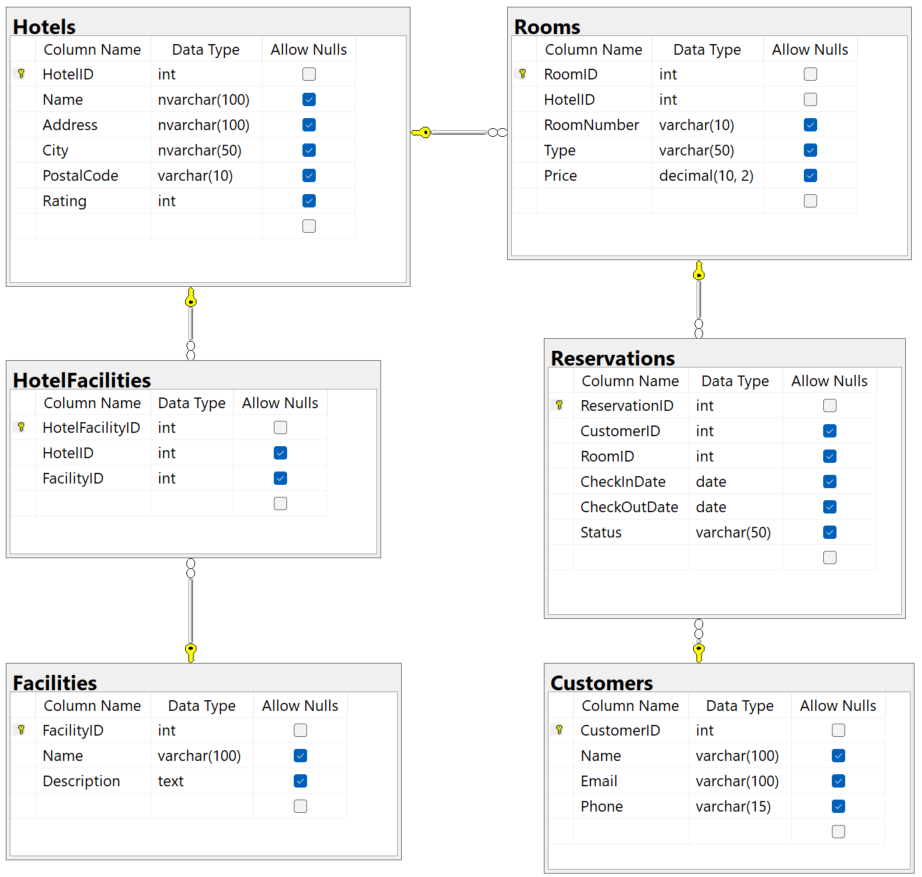
\includegraphics[width=\textwidth]{figures/SWD_ERD_HotelManagement.png}
    \caption{Entity Relationship Diagram}\label{EntityRelationDiagram}
  \end{subfigure}
  \caption{Domain Model and Entity Relationship Diagrams}
\end{figure}

\subsection{Domain Model Diagram}
See Figure 1. This DMD only contains entities, multiplicities, and relationships.
This provides input on how the database should be designed based on the individual tables and their relationships to each other.

\subsection{Entity-Relationship Diagram}
See Figure 1. The ERD is generated from the tables in the database and shows the relationships between the tables, their PK, FK, and data types.
